\documentclass[10pt,a4paper]{article}
\usepackage[utf8]{inputenc}
\usepackage[francais]{babel}
\usepackage[T1]{fontenc}
\usepackage{amsmath}
\usepackage{amsfonts}
\usepackage{amssymb}
\usepackage{makeidx}
\usepackage{graphicx}
\usepackage{float} %pour que l'option "H" fonctionne dans figure.
\usepackage[left=2cm,right=2cm,top=2cm,bottom=2cm]{geometry}
\usepackage{hyperref} % lien hypertext
%\hypersetup{pdfborder={0 0 0}}

\begin{document}
%\setcounter{page}{1} % enlever numero de page


\begin{minipage}{0.5\linewidth} % permet de faire les deux colonnes pour mettre l'image à  droite du texte
Colpier Clément\\
Fornara Thibault\\
Pellegrino Guillaume\\
Renard Charles\\



26/01/13
\end{minipage}
\begin{minipage}{0.5\linewidth}
\begin{flushright}

\includegraphics[scale=0.2]{logo-esiee.jpg}

\end{flushright}
\end{minipage}


\vspace{8cm}

\begin{center}
\LARGE Projet de Mathématiques appliquées \\
\-
\LARGE PR3003
\\

\end{center}




\newpage
-
\newpage
\tableofcontents              % Table des matieres
\clearpage


\section{Déterminer l'équation différentielle vérifiée par M(t)=(x(t),y(t)).}
\begin{figure}[H]
	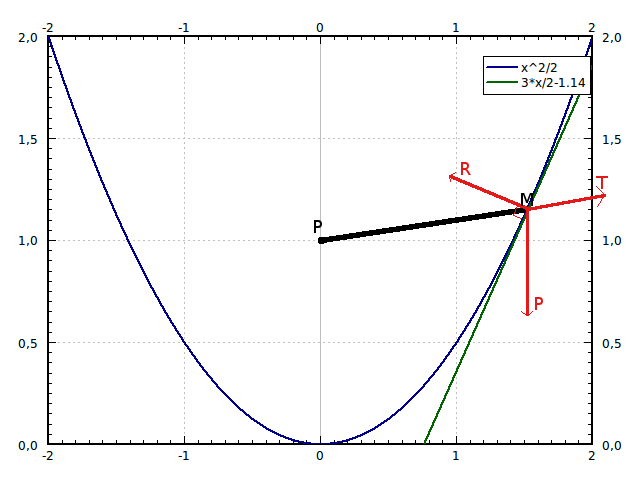
\includegraphics[scale=0.7]{GraphMath2.png}
	%\caption{Histoire de Sanofi}
\end{figure}
La masselotte M se déplace uniquement selon la composante tangentielle. Pour déterminer l'équation différentielle on va donc particulièrement s'intéresser à l'équation sur la composante tangentielle.\\
Pour cela, on commence à faire la somme des forces s'exerçant sur la composante tangentielle $\vec{u_t}$ et normale $\vec{u_n}$:
\[
   \left \{
   \begin{array}{r c l}
      P_t+T_t=ma_t  \\
      P_n+R_n+T_n=0 
   \end{array}
   \right .
\]
On s'intéresse à l'équation: \[\fbox{$P_t+T_t=ma_t$}\] \\ 
Pour déterminer l'équation différentielle, on doit alors projeter $\vec{T}$ et  $\vec{mg}$ sur $\vec{u_t}$. \\
On projette $\vec{mg}=-mg.\vec{u_y}$ sur $\vec{u_t}$\\

\subsubsection{Projection du Poids sur la composante tangentielle}
\begin{figure}[H]
	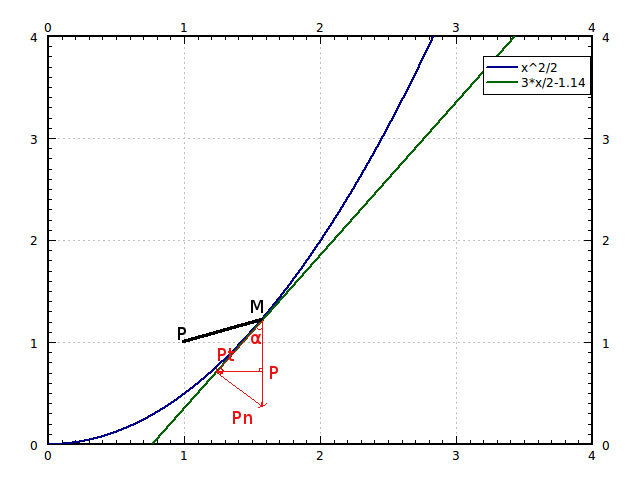
\includegraphics[scale=0.7]{GraphMathZoomProjectionPoids.png}
	%\caption{Histoire de Sanofi}
\end{figure}

On remarque sur le graphique que $P_t=P.\cos(\alpha)$\\
On cherche à déterminer $\alpha$.
On calcule la pente a de la tige parabolique. $a=\frac{\partial y}{\partial x}=\frac{\partial x^2/2}{\partial x}=x$ \\
En $M(x_0,y_0)$ la pente a de la tige parabolique vaut donc $x_0$.
Cette pente a nous permet de calculer l'angle $\alpha$. En effet, on remarque graphiquement que $\tan(\alpha)=\frac{1}{a}$. On en déduit: $\alpha=\tan^{-1}(\frac{1}{x_0})$\\
Au final on trouve donc: $P_t=P.\cos(\tan^{-1}(\frac{1}{x_0})) $\\
Or $\cos(\tan^{-1}(x))=\frac{1}{1+x^2}$  On en déduit donc: $P_t=P.\frac{1}{1+1/x^2_0}$ D'où: 
\[\fbox{$P_t=P.\frac{x_0}{1+x^2_0}$}\]

\subsubsection{Projection de la tension du ressort su la composante tangentielle}
On projette désormais $\vec{T}$ sur $\vec{u_t}$.\\
\begin{figure}[H]
	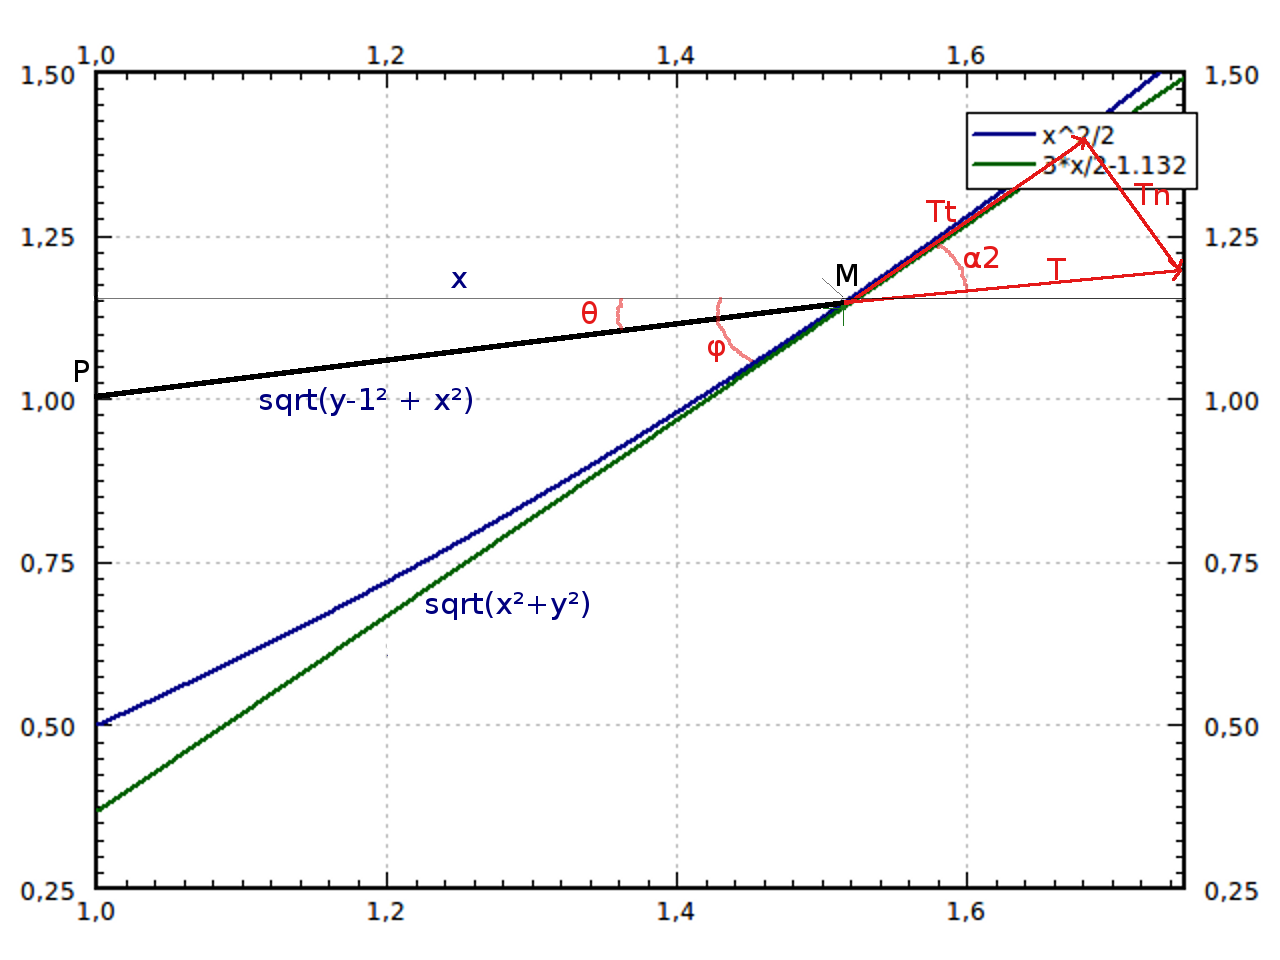
\includegraphics[scale=0.35]{GraphMathZoomProjectionT2.png}
	%\caption{Histoire de Sanofi}
\end{figure} 

$\cos(\phi)=\frac{x}{\sqrt{x^2+y^2}}=\frac{1}{\sqrt{1+x^2}}$ \\

$\cos(\theta)=\frac{x}{\sqrt{(1-y)^2+x^2}}=\frac{x}{\sqrt{1+x^4/4}}$ \\
Et: 
$T_t=T.\cos(\alpha 2)=T.\cos(\phi - \theta)=T[\cos(\phi).\cos(\theta)+\sin(\phi).\sin(\theta)]$\\
On en déduit:\\
$T_t=T[\frac{1}{\sqrt{1+x^2}}.\frac{x}{\sqrt{1+x^4/4}} + \sin(\cos^{-1}(\frac{1}{\sqrt{1+x^2}})).\sin(\cos^{-1}(\frac{x}{\sqrt{1+x^4/4}}))]$\\
Or: $\sin(\cos^{-1}(u))=\sqrt{1-u^2}$\\
On trouve donc:\[\fbox{$T_t=T.[\frac{1}{\sqrt{1+x^2}}.\frac{x}{\sqrt{1+x^4/4}} + \sqrt{1-\frac{1}{1+x^2}}.\sqrt{1-\frac{x^2}{1+x^4/4}}]$}\]\\

%La pente de la tangente vaut $x_0$. Celle de $\vec{PM}$ vaut $\frac{y_0-1}{x_0}$.\\
%On en déduit ainsi: $\tan(\phi)=x_0$ et $\tan(\theta)=\frac{y_0-1}{x_0}$
%On obtient ainsi $\alpha=\tan^{-1}(x_0) - \tan^{-1}(\frac{y_0-1}{x_0})$ et on en déduit: $T_t=T.\cos(\tan^{-1}(x_0) - \tan^{-1}(\frac{y_0-1}{x_0}))$ \\

\subsubsection{Détermination de $a_t$}
On a vu dans la première équation que $a_n=0$. On en déduit: $||\vec{a}||=a_t$
On peut ainsi écrire: $a_t=||\vec{a}||$\\ %=$\sqrt{a_x^2+a_y^2}$
Or $||\vec{a}||=\frac{\partial v}{\partial t}=\frac{\partial \sqrt{\dot{x}^2+\dot{y}^2}}{\partial t}$\\
On trouve: \[\fbox{$a_t=\ddot{x}.\sqrt{1+x^2}+ \frac{\dot{x}^2.x}{\sqrt{1+x^2}}$}\] %(Equation de Charles)
%On obtient alors: $a_t=\sqrt{\ddot{x}^2+\ddot{y}^2}$

\subsubsection{Détermination de l'équation différentielle}
A l'aide de ce qu'on a calculé précédemment on développe l'équation $mg_t+T_t=ma_t$ pour déterminer l'équation différentielle.
On obtient alors: 
\[\fbox{ $mg.\frac{x}{1+x^2} + k(l-l_0).[\frac{1}{\sqrt{1+x^2}}.\frac{x}{\sqrt{1+x^4/4}} + \sqrt{1-\frac{1}{1+x^2}}.\sqrt{1-\frac{x^2}{1+x^4/4}}] - m\ddot{x}.\sqrt{1+x^2} - \frac{m\dot{x}^2.x}{\sqrt{1+x^2}} = 0$}\]
% \[mg.\cos(\tan^{-1}(x_0)) + k(l-l_0).\cos(\tan^{-1}(x_0) - \tan^{-1}(\frac{y_0-1}{x_0}))=\sqrt{\ddot{x}^2+\ddot{y}^2}\]
 %En développant on a:\[mg.\cos(\tan^{-1}(x)) + k(\sqrt{(x^2/2-1)^2+x^2}-l_0).\cos(\tan^{-1}(x) - \tan^{-1}(\frac{x^2/2-1}{x})) - \sqrt{\ddot{x}^2+1}=0\]

%Equa diff de Charles:
%\[ \fbox{$ \ddot{x}.\sqrt{1+x^2}+ \frac{5x^3/8 + x^2/4 + \dot{x}.x}{1+x^2} + \frac{x}{\sqrt{1+x^2}} - \frac{l_0(5x^3/4 + x^2/2)}{2\sqrt{1+x^4/4}\sqrt{1+x^2} }=0 $}\]




\end{document} 